\documentclass{beamer}

\title{PageRank}
\author{Ben Burns, Dan Magazu, Lucas Chagas, \\Thomas Webster, Trung Do}
\date{Fall 2021}

\usepackage{outlines}
\usepackage{graphicx}
\usepackage{amsmath}
\usepackage{color, xcolor, mdframed}

\graphicspath{{./images}}

\addtobeamertemplate{navigation symbols}{}{
    \usebeamerfont{footline}
    \usebeamercolor[fg]{footline}
    \hspace{1em}
    \insertframenumber/\inserttotalframenumber
}

%\AtBeginSection[ ]
%{
%\begin{frame}{Outline}
%    \tableofcontents[currentsection]
%\end{frame}
%}

\begin{document}

\frame{\titlepage}

\begin{frame}
\frametitle{Table of Contents}
\tableofcontents
\end{frame}

\section{Background}
\begin{frame}[t]{PageRank}
\begin{outline}
    \1 PageRank is the algorithm to determine the importance of a website relatively to all other websites. The algorithm ranks the importance of website $w,$ i.e., PR($w$), based on the number of links points to website w and the \emph{quality} of each pointing link from the other source website. 

    \1 \textbf{The underlying assumption}: More important website are likely to receive more links from other website. Since the algorithm measures the relative popularity ("ranking") between all websites, websites with higher ranking score are ranked higher. The sum of all ranking score equals 1 (will see why later).
\end{outline}
\end{frame}

\section{Formalizing PageRank}
\begin{frame}[t]{Formalizing the PageRank problem}
\begin{outline}
    \begin{columns}
        \begin{column}{0.5\textwidth}
            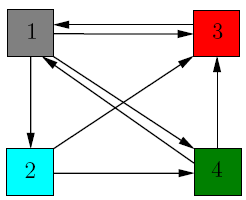
\includegraphics[width=\textwidth]{unweighted.png}
        \end{column}
        \begin{column}{0.5\textwidth}
            As a graph: Each website is represented by a node assigned with a PageRank value, denoted by PR(w). If a website w has a link to another website v (meaning there are an outbound link from w and an inbound link to v), then there is a directed edge from node w to node v. Multiple links from w to v is treated as a single edge from node w to v, and all self-links from a website to itself are ignored. Thus, this is a node-weighted, simple, no self-loop directed graph.
        \end{column}
    \end{columns}
\end{outline}
\end{frame}

\begin{frame}
\frametitle{Edge Weights}
\begin{columns}
    \begin{column}{0.5\textwidth}
        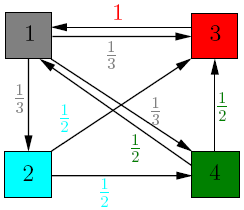
\includegraphics[width=\textwidth]{weighted.png}
    \end{column}
    \begin{column}{0.5\textwidth}
        This edge has its weight equal to PR(*w*) divided by the total number of outbound links of $w$, L($w$). Then recipient node $v$ "receives" the PageRank value of $w$, adding to its own value, i.e., PR($v$) += PR($w$)/L($w$). 
        
        In another words, for a given node in the graph:

        \textbf{An outbound link} will "give" away the PR value of the source node to the recipient node.  

        \textbf{An inbound link} will add the PR value from the source node to the recipient node.
    \end{column}
\end{columns}
\end{frame}

\begin{frame}[t]{Perspectives for Solving}
    \begin{itemize}
        \setlength\itemsep{1em}
        \item There are two ways to understand the problem:
        \item[1)] as an Eigenvector problem
        \item[2)] as a probability problem
        \item Both perspectives use linear algebra 
    \end{itemize}
\end{frame}

%\begin{frame}{Adjacency Matrix}
%\begin{columns}
%    \begin{column}{0.5\textwidth}
%        \centering
%        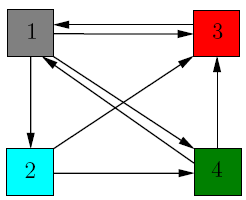
\includegraphics[width=\textwidth]{unweighted.png}
%    \end{column}
%    \begin{column}{0.5\textwidth}
%        \centering
%        {\Large$A = \begin{pmatrix}
%            0 & 1 & 1 & 1\\
%            0 & 0 & 1 & 1\\
%            1 & 0 & 0 & 0\\
%            1 & 0 & 1 & 0\\
%        \end{pmatrix}$}
%    \end{column}
%\end{columns}
%\begin{outline}
%    \1 No self loops means the main diagonal is all zeros
%\end{outline}
%\end{frame}

\begin{frame}[t]{Eigenvector Problem}

\end{frame}

\begin{frame}[t]{Probability Problem}

\end{frame}

\begin{frame}[t]{Power Iteration}

\end{frame}

\begin{frame}[t]{Spider Traps and Deadends}

\end{frame}

\begin{frame}[t]{Random Teleports + Damping factor}
    
\end{frame}

\begin{frame}[t]{The solution to the Spider traps}
    \begin{itemize}
        \item At each time step, the random surfer chooses 1 of 2 options:
        \item With some probability $\beta$, the surfer will follow a random link
        \item With the remaining probability 1 -$\beta$ , the surfer will jump to random page
        \item This means within a few time steps, the surfer will teleport out of the spider trap within a few time steps
    \end{itemize}
\end{frame}
    
\begin{frame}[t]{The Solution to Dead Ends}
\begin{outline}
\1 Dead end problem: the pages that have zero scores, which leads to their PageRank score not getting distributed to any other page in the graph, not pointing to any other graph
\1 After running the power iteration, after several iterations, it will converge towards zero, which leads to the PageRank score of a particular node not being passed down and leaking out of the system
\1 How to solve the Dead Ends Problem:
        \2 Solution: Always Teleports
        \2 If a node has no outgoing links, when we reach that node, we teleport with a probability of 1
        \2 this means that whenever we reach the dead-end node, we will always jump out and reach somewhere else
\end{outline}
\end{frame}
    
\begin{frame}[t]{Why Do Teleports Solve the problem?}
\begin{outline}
\1 For any start vector, the power method applied to a Markov transition matrix A will converge to a unique positive stationary vector as long as A is stochastic, irreducible, and aperiodic.
    \2 Stochastic: Every column in the transition matrix sums to 1
    \2 Aperiodic: A chain is periodic if there exist k > 1 such that the interval between two visits to some state s is always a multiple of k
    \2 Irreducible: From any state, there is a non-zero probability of going from any one state to another
\end{outline}
\end{frame}
    
\begin{frame}[t]{The PageRank equation}
\begin{outline}
\1 Google's solution makes the Markov Transition matrix stochastic, aperiodic, and irreducible.

\1 PageRank equation:

\begin{mdframed}[backgroundcolor=blue!20]
    \begin{center}
        $r_j = \sum\limits_{i\to j}\beta \dfrac{r_i}{d_i} + (1-\beta)\dfrac{1}{n}$
    \end{center}
\end{mdframed}

\2 The summation is the sum of all of the importance of node $I$ that point to it where $r_j$ and $r_i$ is the probability that the random surf is on this node.
\2 This is divided by $d_i$, which is the probability that the random surf traverses the link when iterating towards $j$. This only happens with probability $\beta$, when the surfer decides to follow the link.
\2 The $(1-\beta)/n$ represents when the random walkers decide to jump somewhere else, using the probability ($1-\beta) \cdot 1/n$, where $n$ is the number of nodes in the entire network.
\end{outline}
\end{frame}

\end{document}